\chapter{Evaluation}
\label{chapter:evaluation}
\minitoc\vspace{.5cm}
% In this chapter the implementation of Component X is evaluated. An example instance
% was created for every service. The following chapter validates the component implemented
% in the previous chapter against the requirements.
% Put some screenshots in this section! Map the requirements with your proposed solution.
% Compare it with related work. Why is your solution better than a concurrent
% approach from another organization?
In this chapter the implementation of the plugins, based on the previously defined requirements and concepts, are evaluated.
Therefore several performance tests will be analyzed and the code verification will be shown.
Afterwards the final system is demonstrated.

\section{Test Environment}
\label{section:test-environment}
Motey and the performance scripts in section \ref{section:performance-evaluation} was tested on three different devices.
\begin{enumerate}
  \item \textbf{Raspberry Pi 2 Model B Version 1.1} hereinafter called \textbf{NeoPi}, that has a ARM Cortex-A7 \ac{CPU} with four cores each with 900 MHz and a 32-bit architecture. It has 1024 MB \ac{RAM} and a 10/100-MBit-Ethernet port. The device is running a Raspbian 8 (jessie) with Linux Kernel version 4.9.
  \item \textbf{Raspberry Pi 3 Model B Version 1.2} hereinafter called \textbf{BuffPi}, is the currently the newest Raspberry Pi on the market. It has a ARM Cortex-A53 \ac{CPU} also with four cores, but each has 1200 MHz and 64-bit architecture. It also has 1024 MB \ac{RAM} and a 10/100-MBit-Ethernet port.  This devices is also runngin Raspbian 8 (jessie) with Linux Kernel version 4.9.
  \item \textbf{Acer Aspire V5-573G} hereinafter called \textbf{Laptop}, with an Intel Core i7-4500U \ac{CPU} with two cores each 1.80 GHz and a 64-bit architecture as well. It has 8 GB \ac{RAM} and a 802.11n WiFi connection. It is running a Linux Mint 18.1  64-bit \ac{OS} with a Linux Kernel version 4.4.
\end{enumerate}

Both the \textit{NeoPi} and the \textit{BuffPi} are connected via ethernet to a router.
The \textit{Laptop} is connect via 802.11n WiFi to the router.
% TODO: network information, multiple devices, etc.

\section{Performance Evaluation}
\label{section:performance-evaluation}
In the following section some performance relevant tests are shown and analyzed.
Especially the performance of the used virtualization method is crucial for the system as well as the connection performance of the used protocols are important.
All evaluations are made with low-power devices in mind.
This means a small overhead and a fast and leightweight solution is preferred.

\subsection{Docker vs. KVM}
Due to the fact that Docker is the main component in the created prototype, it is important to verify the performance on low-power devices.
Unfortunately a performance comparison with established \ac{VM} tools like VMWare or Xen on a Raspberry Pi is not possible, because nearly all of them does not support the ARM \ac{CPU} architecture.
There are several performance tests on x86 architecture.
IBM for example compared \acp{VM} or more specific \acp{KVM} with Docker in a research report\autocite{IBM:Performance:2014} from 2014.
They conclusion was that \ac{KVM} has a significant overhead to every I/O operation.
Therefore it is less suiteable for latency-sensitive workloads or high I/O rates.
Figure \ref{fig:ibm_kvm_docker_io} show the throughput for random I/O operations for a native, a Docker virtualized and a \ac{KVM} virtualized system.

\begin{figure}[H]
    \centering
    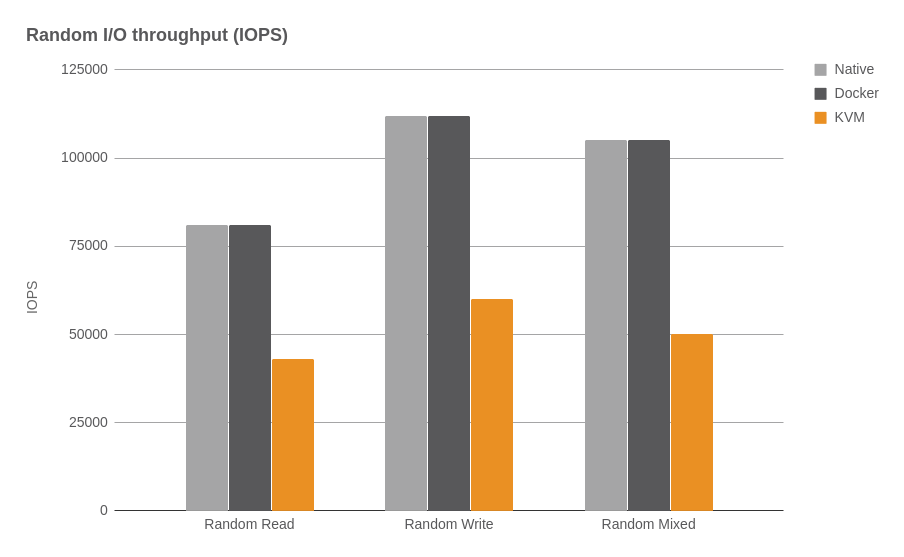
\includegraphics[width=\textwidth]{resources/images/performance_ibm_kvm_docker_io.png}
    \caption[KVM and Docker I/O throughput comparison by IBM]{KVM and Docker I/O throughput comparison by IBM. Adapted from: \autocite[p. 6]{IBM:Performance:2014}}
    \label{fig:ibm_kvm_docker_io}
\end{figure}

Compared to the native system, Docker has "nearly no overhead"\autocite[p. 6]{IBM:Performance:2014}.
But also Docker has some drawbacks.
For example it has an overhead for workloads with high packet rates.\autocite[cf.][p. 6]{IBM:Performance:2014}
The overall conclusion by IBM was that Docker is more performant than a \ac{KVM} virtualized system.

Another benchmarking comparison\autocite{Russell:Performance:2014} between Docker and \ac{KVM} that was also made by IBM show a much clearer result.
In this test Docker is much more performant in nearly every point of view.
It has less overhead in terms of \ac{CPU} usage\autocite[cf.][p. 25]{Russell:Performance:2014}, memory performance\autocite[cf.][p. 50]{Russell:Performance:2014} and boot time\autocite[cf.][p. 24]{Russell:Performance:2014}.
Only the network troughput is nearly the same.\autocite[cf.][p. 52]{Russell:Performance:2014}
Finally also the container size is much smaller in Docker than in \ac{KVM}.\autocite[cf.][p. 66]{Russell:Performance:2014}
Overall Docker is much more lightweight and due to the fact that it supports the ARM architecture, it is well suiteable for the usage on low-power devices.

\subsection{Performance HTTP}
To test the \ac{HTTP} performance of the application two simplified test scripts are created.
Both are located in the \textit{performance\_tests/http} folder in the motey project.
The \textit{server.py} script starts a Flask server and waits for a POST request.
If it gets one it will send back a static container id.
The \textit{client.py} script is used to send the \ac{JSON} data to the server.
It is an extract of an Docker image command as it would be used in the Motey application.
Afterwards 10.000 request will be send to the server.
This execution is one iteration of the test.
In total 10 iterations are performed to get an result.
An overview of all test results are shown in section \ref{appendix:http_test_results}.
Figure \ref{fig:performance_http_server_comparison} shows the result of the tests.

\begin{figure}[H]
    \centering
    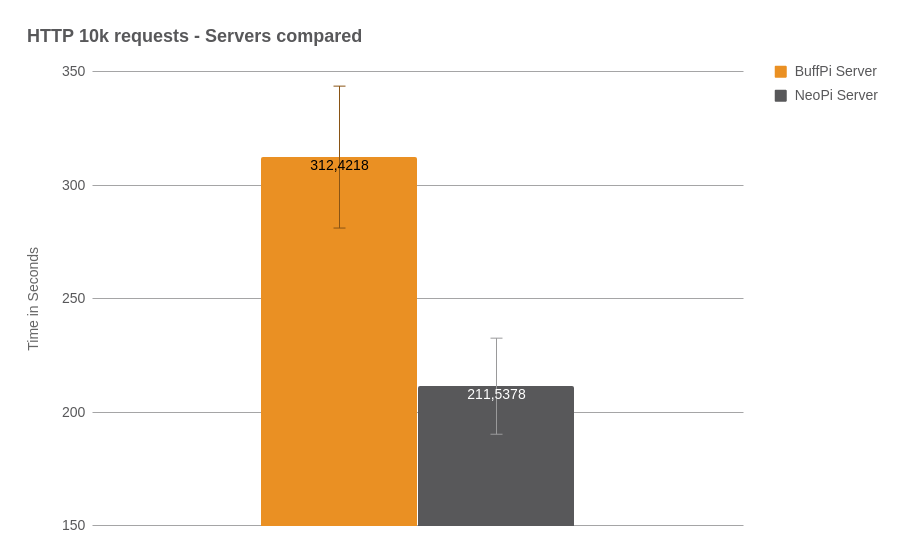
\includegraphics[width=\textwidth]{resources/images/performance_http_server_comparison.png}
    \caption[HTTP 10k requests - Server comparison]{HTTP 10k requests - Server comparison}
    \label{fig:performance_http_server_comparison}
\end{figure}

There are two bars indicating the time needed to send 10.000 requests: the left one, that represents a setup where the more powerful BuffPi was the server and the NeoPi was the client, tokes in total more time, then the setup where the NeoPi is the server.
This is a suprising outcome because the assumtion was that the server tokes more computation time then the client.
But the results prove the opposite.
If the less powerful device is the server the packages are much faster sent the vice versa.
Overall using \ac{HTTP} as the protocol of choice, the messaging is pretty slow.
To send the 10.000 request even the faster setup toke 03:31 minutes.
This result depends on the huge package overhead in \ac{HTTP} and also the need for waiting for the request.
Such a setup is fits well for simple status or rarely sent deployment requests, but not for high frequently used inter-node connections or in a low latency environment.

\subsection{Performance ZeroMQ}
Also for the ZeroMQ performance test both Raspberry Pis are used to communicate with each other.
Similar to the \ac{HTTP} test the BuffPi and the NeoPi are switch between server and client.
To test the ZeroMQ performance, the test has to be splitted up into two different variants.
The first one is called \textit{\ac{CC}}.
This means, once a ZeroMQ connection is established, all of the 10.000 request are send via this one session.
\textit{\ac{NC}} is used to simulate the case where each connection has to be closed before a new request will be send.
This is more realistic to the implementation in Motey, because the connection to one node will established in the moment they are needed and closed as soon as the request is done.
Beside that the test setup is the same like in the \ac{HTTP} performance test.
The scripts are located in \textit{performance\_tests/zeromq} folder, the \textit{server.py} script is the same for both variant, only the client scripts differ.
Each client send out 10.000 requests and each iteration is performed ten times.
The total test results are in section \ref{appendix:zeromq_test_results}.

\begin{figure}[H]
    \centering
    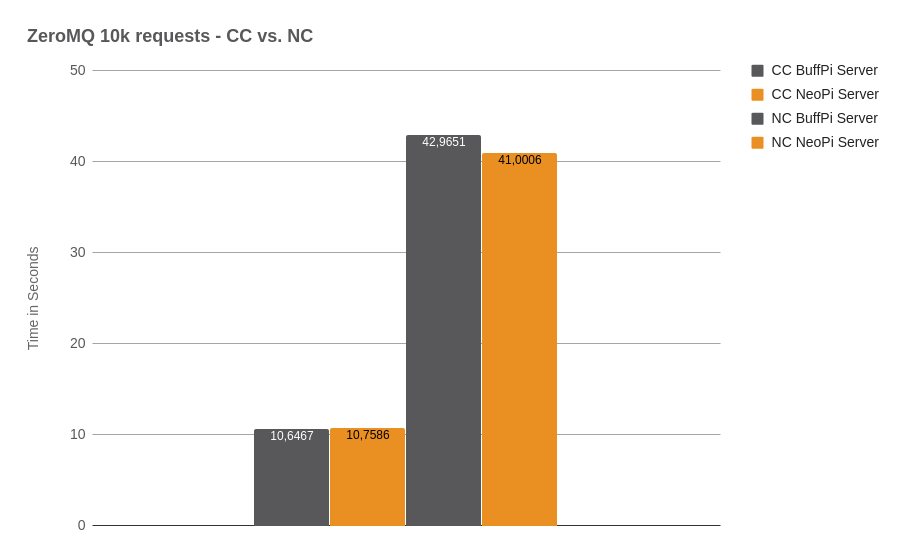
\includegraphics[width=\textwidth]{resources/images/performance_zeromq_cc_vs_nc.png}
    \caption[ZeroMQ comparison between new connection and constant connections]{ZeroMQ comparison between new connection and constant connections}
    \label{fig:performance_zeromq_cc_vs_nc}
\end{figure}

The difference between the \ac{CC} and \ac{NC} is significant.
The \ac{CC} is around four times faster then the \ac{NC}.
Certainly this relates to the connection and deconnection phase of the socket.
On the other side the difference between the two devices is minimal and can be neglected in this evaluation.

The comparison between ZeroMQ and \ac{HTTP} is much more crucial.
Compared to the \ac{CC} \ac{HTTP} is around 20 times slower.
Even compared to the \ac{NC} it is around 5 times slower.
Figure \ref{fig:performance_zeromq_vs_http} shows the test results.

\begin{figure}[H]
    \centering
    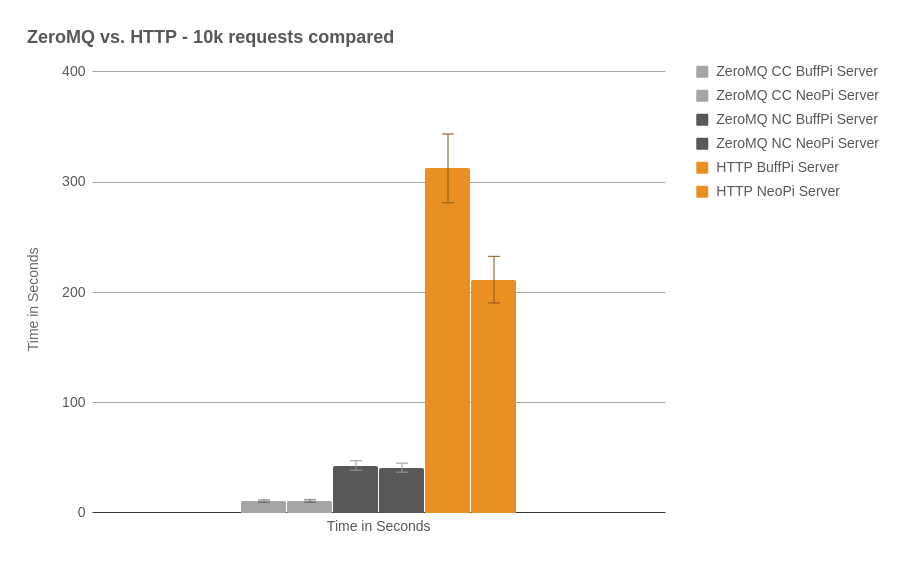
\includegraphics[width=\textwidth]{resources/images/performance_zeromq_vs_http.png}
    \caption[Performance comparison ZeroMQ vs. HTTP]{Performance comparison ZeroMQ vs. HTTP}
    \label{fig:performance_zeromq_vs_http}
\end{figure}

In addition to that \ac{HTTP} have a huge packet overhead that will consume more network bandwidth.
ZeroMQ is well suiteable for low latency connections and on the same side more lightweight.
In the test ZeroMQ is always used in \ac{TCP} mode.
The creator of ZeroMQ promise that the \ac{IPC} and especially the inter-thread protocol are much faster than \ac{TCP}.\autocite[cf.]{ZeroMQ:UicastTransports}
But still for the \ac{TCP} mode, the results are self-evidently.


\subsection{Performance MQTT}
% versuchsaufbau erklären
% daten format erklären
% das es 10 durchläufe waren erklären
% auf Problem mit packet loss eingehen
% -> puffer muss groß genug sein
% Diagram auswerten
% -> auf QoS level eingehen
% ---> unterschied significant
% ---> mehr als doppelt so lang zwischen QoS 0 und QoS 2
% ---> verglichen zu HTTP immer noch sehr schnell

% -> Broker Device eingehen
% ---> langsamer Broker führt zu schlechterem Durchsatz
% ---> selbst langsames Device noch gute werte verglichen zu HTTP
% ---> Dennoch wichtig
% ---> Empfehlung: Startes device aka Cloud for MQTT
\begin{figure}[H]
    \centering
    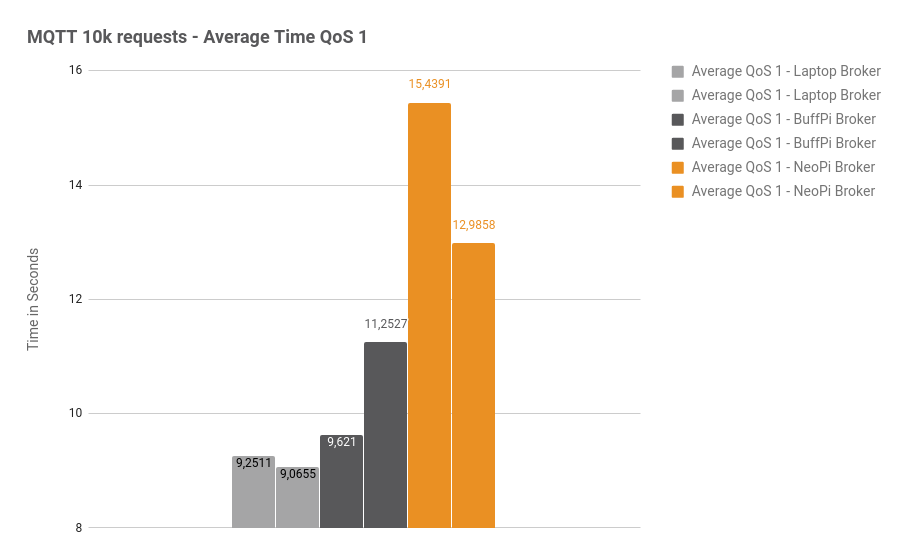
\includegraphics[width=\textwidth]{resources/images/performance_mqtt_average_time_qos_1.png}
    \caption[MQTT average time for QoS 1]{MQTT average time for QoS 1}
    \label{fig:performance_mqtt_average_time_qos_1}
\end{figure}
\begin{figure}[H]
    \centering
    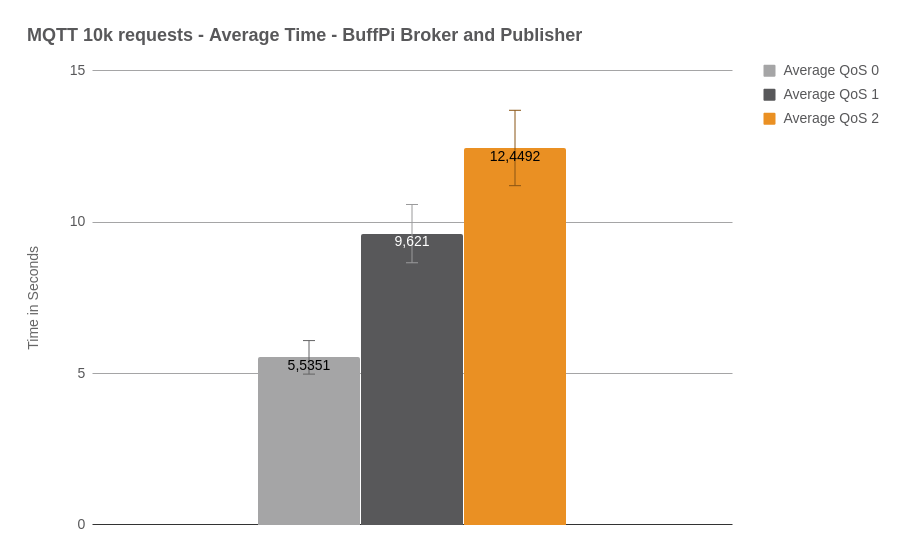
\includegraphics[width=\textwidth]{resources/images/performance_mqtt_average_time.png}
    \caption[MQTT average time for all QoS levels]{MQTT average time for all QoS levels}
    \label{fig:performance_mqtt_average_time_all_qos}
\end{figure}


\section{Scalability}
\label{section:scalability}
% MQTT maximum
% weitere nodes hinzufügen
% existierende entfernen
% Docker Container maximum
\doit

\section{Code Verification}
\label{section:code-verification}
Code verification is a quite important technique in every development project.
There are several possibilities to check and verify the integrity of the created source code.
Two of them are used in this project.
The style check is used to ensure the compliance with the code style guidelines and the unit tests are used to verify the correctness of the code and the outcome of the functions itself.
As the guidelines the pretty famous \ac{PEP} 8 style guide\footnote{\url{https://www.python.org/dev/peps/pep-0008}} is used.
\ac{PEP} 8 is used in the Python standard library code and is well established in the community.
A standardized code style is recommended in team projects as well as in open source projects.
But also in private project a commitment to a specific style can be helpful to make the project easier to maintain.
The code in general becomes more readable, more understandable and the amount of errors can be decreased.
Due to the fact that overall code is read more often than it is written, other people will be satisfied by having a common understanding of the "grammar" of the code to be used.
As the tool of choice the library \textit{pycodestyle} will be used.
The style check is part of the \ac{CI} pipeline and the concrete implementation was shown in listing \ref{code:travis_config}.
If there is any style check violation, the \ac{CI} build process will fail and the new Docker image will not be uploaded.

\begin{listing}[H]
  \begin{minted}{bash}
  $ pycodestyle --ignore=E241,E501 motey/
  motey/di/app_module.py:48:38: E128 continuation line under-indented for visual indent
  motey/di/app_module.py:49:38: E128 continuation line under-indented for visual indent
  motey/di/app_module.py:50:38: E128 continuation line under-indented for visual indent
  motey/di/app_module.py:51:38: E128 continuation line under-indented for visual indent
  motey/di/app_module.py:52:38: E128 continuation line under-indented for visual indent
  motey/di/app_module.py:53:38: E128 continuation line under-indented for visual indent
  motey/di/app_module.py:54:38: E128 continuation line under-indented for visual indent
  motey/configuration/configreader.py:6:66: E703 statement ends with a semicolon

  The command "pycodestyle --ignore=E241,E501 motey/" exited with 1.

  $ pycodestyle --ignore=E241,E501 samples/

  The command "pycodestyle --ignore=E241,E501 samples/" exited with 0.
  \end{minted}
  \caption[Sample output of the style check validation from the Travis \ac{CI} build process number 148]{Sample output of the style check validation from the Travis \ac{CI} build process number 148\autocite{Travis:Build:148}}
  \label{code:style_check_validation}
\end{listing}

Listing \ref{code:style_check_validation} shows an example output of the Travis \ac{CI} build process.
The first style check call fails due to multiple validations, but the second one exited successfully.\newline

The second verification is are the unit tests.
A unit test is as the name implies a software test method which tests each component of an application.
Each component should be tested as isolated as possible by invoking only one or a couple of methods from a unit and the result should be verified automatically and compared with an expected result.\autocite[cf.][p. 320]{Olan:2003:UTT}
All the used objects in a class should be as independent from each other as possible.
To ensure this, the objects have to be mocked by a mocking framework.
The python unit test framework has a build-in mocking framework since version 3.
A mock is a fake objects that acts as a dummy for the class to be tested.
To decouple the dependencies and to increase the testability and more specific to make used object easier mockable, the \ac{DI} pattern is used.
Each injected object can be easily mocked outside of the class.
Due to the fact that Python allows to modify each class member at any time, \ac{DI} is not really necessary, but it helps to make it clearer to understand and the code more readable and maintainable.\newline

The advantages of unit tests in general are that problems can be easier localized and much faster detected.
If an error occures during unit testing a former well working code, it is obvious that the last code changes are the reason for the error.
This benefit is also helpful to readuce the fear of refactoring or extend code parts.
Even pretty old parts of an application can be modified without the risk of any major problems.
When the unit test are part of the \ac{CI}, each build will be checked.
This reduces the risk of the deployment of faulty code.
And finally unit tests can be a good starting point for new team members, because it helps to understand the functionality of a class.
An unit test can acts as some kind of documentation.
The downsides are that unit tests are coded.
This means also unit tests can have errors.
Furthermore poorly written unit tests or tests that a written unpleasured can end up in a wrong feeling of safeness.
Some error case could not be catched and the submitted code is still faulty.
Additionally the test setup is not realistic.
Integration test are more accurate in terms of the human behavior.
Also the dependencies between the component and the interaction between them can be tested much better with integration test.
The most critical part of unit test in the economy is that the take time.
For each written component, the realted tests take a significant time to be developed.
In a real life project this could be unacceptable even if it is important to have them.\newline

\begin{listing}[H]
  \begin{minted}{python}
  class TestServiceRepository(unittest.TestCase):
    @classmethod
    def setUp(self):
        self.text_service_id = uuid.uuid4().hex
        self.test_service = {'id': self.text_service_id, 'service_name': 'test service name', 'images': ['test image']}
        service_repository.config = {'DATABASE': {'path': '/tmp/testpath'}}
        service_repository.BaseRepository = mock.Mock(service_repository.BaseRepository)
        service_repository.TinyDB = mock.Mock(TinyDB)
        service_repository.Query = mock.Mock(Query)
        self.test_service_repository = service_repository.ServiceRepository()

    def test_has_entry(self):
        self.test_service_repository.db.search = mock.MagicMock(return_value=[1, 2])

        result = self.test_service_repository.has(service_id=self.test_service['id'])

        self.assertTrue(self.test_service_repository.db.search.called)
        self.assertTrue(result)
  \end{minted}
  \caption{Extract from the Motey unit test of the ServiceRepository}
  \label{code:sample_unit_test}
\end{listing}

% TODO
\todo{describe the listing}\newline

Unit testing in general can be realized in two different ways.
The first possibility is the by writing the tests after the code is done.
\todo{finalize this paragraph}\newline

The second possibility is the \ac{TDD}, that is related to the test-first programming concept of the extreme programming development.
In this development methodology the tests are written before the implementation of a class is created.
This helps to plan the architecture of a class and catch edge cases before the implementation is done.
\ac{TDD} is an iterative process where at first the test is written, then the test will be executed and must fail, afterwards the code is written and the tests should be executed again, but this time successfully.
Finally the process can be repeated for example if the code has to be refactored or extended.
Especially in an extrem programming environment \ac{TDD} in combination with pair programming and code reviews are reasonable.\newline

Motey was created with the "normal" unit testing approach, due to the fact that it was a one man project with rapidly changing requirements and an explorative approach to create the prototype.
Nevertheless both methods ends up in a well tested code base and an assured code stability.

\section{Conclusion}
\doit
